\def\apname{Приложение. PDDL-описания предметных областей и задач планирования и сгенерированные для них UML-модели}

\chapter*{\apname}
\addcontentsline{toc}{chapter}{\apname}

\def\sname{1. Предметная область ``Логистика''}
\section*{\sname}

\begin{mdframed}[style=excode] 
\begin{alltt}
\small
(define (domain logistics)
  (:requirements :strips :typing)
  (:types 
    package location vehicle - object
    truck airplane - vehicle
    city airport - location)
  
  (:predicates  
        (at ?vehicle-or-package - (either vehicle package) 
            ?location - location)
        (in ?package - package ?vehicle - vehicle)
        (in-city ?loc-or-truck - (either location truck) ?citys - city)
        )
        
  (:action load-truck
    :parameters
         (?obj - package
          ?truck - truck
          ?loc - location)
    :precondition
        (and    (at ?truck ?loc) 
            (at ?obj ?loc))
    :effect
        (and    (not (at ?obj ?loc)) 
            (in ?obj ?truck)))

  (:action load-airplane
    :parameters
        (?obj - package
         ?airplane - airplane
         ?loc - airport)
    :precondition
        (and
            (at ?obj ?loc) 
            (at ?airplane ?loc))
    :effect
        (and    (not (at ?obj ?loc)) 
            (in ?obj ?airplane)))

  (:action unload-truck
    :parameters
        (?obj - package
         ?truck - truck
         ?loc - location)
    :precondition
        (and    (at ?truck ?loc) 
            (in ?obj ?truck))
    :effect
        (and    (not (in ?obj ?truck)) 
            (at ?obj ?loc)))

  (:action unload-airplane
    :parameters
        (?obj - package
         ?airplane - airplane
         ?loc - airport)
    :precondition
        (and    (in ?obj ?airplane) 
            (at ?airplane ?loc))
    :effect
        (and 
            (not (in ?obj ?airplane)) 
            (at ?obj ?loc)))

  (:action drive-truck
    :parameters
        (?truck - truck
         ?loc-from - location
         ?loc-to - location
         ?city - city)
    :precondition
        (and    (at ?truck ?loc-from)
            (in-city ?loc-from ?city)
            (in-city ?loc-to ?city))
    :effect
        (and    (not (at ?truck ?loc-from)) 
            (at ?truck ?loc-to)))

  (:action fly-airplane
    :parameters
        (?airplane - airplane
         ?loc-from - airport
         ?loc-to - airport)
    :precondition
        (at ?airplane ?loc-from)
    :effect
        (and    (not (at ?airplane ?loc-from)) 
        (at ?airplane ?loc-to)))
)

\end{alltt}
\end{mdframed}

Диаграмма фрагмента получившейся модели предметной области:\\

\centerline{
    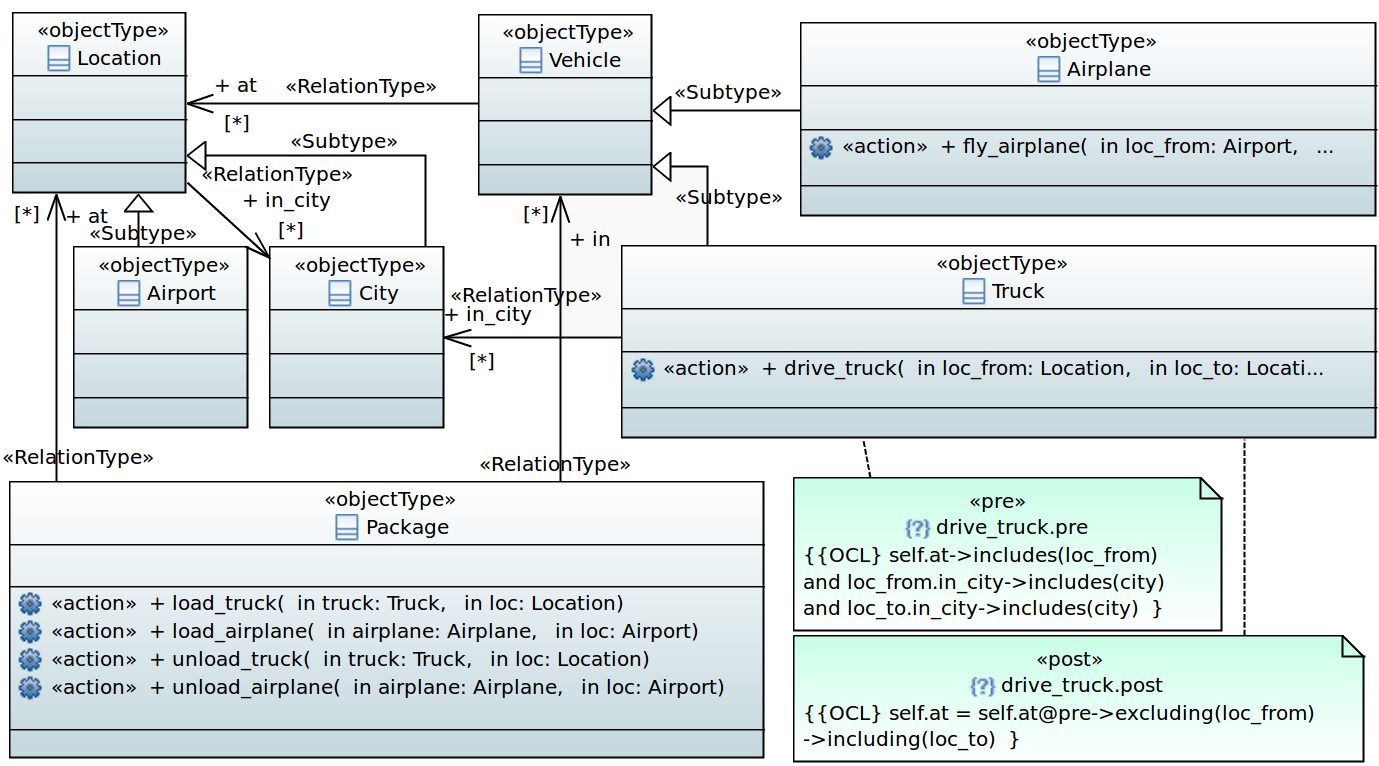
\includegraphics[width=1.2\linewidth, angle=90]{a-logistics-domain}
}

\newpage

\def\sname{2. Предметная область ``Обедающие философы''}
\section*{\sname}

\begin{mdframed}[style=excode] 
\begin{alltt}
(define (domain philosophers)
    (:requirements :typing :negative-preconditions)
    (:types
      Philosopher - object
      Fork - object
    )
    (:predicates
      (right ?phi - Philosopher ?for - Fork)
      (left ?phi - Philosopher ?for - Fork)
      (hold ?phi - Philosopher ?for - Fork)
      (hungry ?phi - Philosopher)
      (hasLeft ?phi - Philosopher)
      (eat ?phi - Philosopher)
      (think ?phi - Philosopher)
      (hasRight ?phi - Philosopher)
    )
    (:action getLeft
     :parameters (?p1 - Philosopher 
                  ?p2 - Philosopher ?f - Fork)
     :precondition 
       (and
         (left ?p1 ?f)
         (right ?p2 ?f)
         (hungry ?p1)
         (not (hold ?p2 ?f))
       )
     :effect
       (and
         (hasLeft ?p1)
         (hold ?p1 ?f)
         (not (hungry ?p1))
       )
    )

    (:action getRight
     :parameters (?p1 - Philosopher 
                  ?p2 - Philosopher ?f - Fork)
     :precondition 
       (and
         (right ?p1 ?f)
         (left ?p2 ?f)
         (hasLeft ?p1)
         (not (hold ?p2 ?f))
       )
     :effect
       (and
         (not (hasLeft ?p1))
         (hold ?p1 ?f)
         (eat ?p1)
       )
    )

    (:action goHungry
     :parameters (?p - Philosopher)
     :precondition 
       (think ?p)
     :effect
       (and
         (not (think ?p))
         (hungry ?p)
       )
    )

    (:action releaseLeft
     :parameters (?p - Philosopher ?f - Fork)
     :precondition 
       (and
         (eat ?p)
         (hold ?p ?f)
         (left ?p ?f)
       )
     :effect
       (and
         (not (hold ?p ?f))
         (not (eat ?p))
         (hasRight ?p)
       )
    )

    (:action releaseRight
     :parameters (?p - Philosopher ?f - Fork)
     :precondition 
       (and
         (hold ?p ?f)
         (right ?p ?f)
         (hasRight ?p)
       )
     :effect
       (and
         (think ?p)
         (not (hold ?p ?f))
         (not (hasRight ?p))
       )
    )

)
\end{alltt}
\end{mdframed}


Диаграмма фрагмента получившейся модели предметной области:\\

\centerline{
    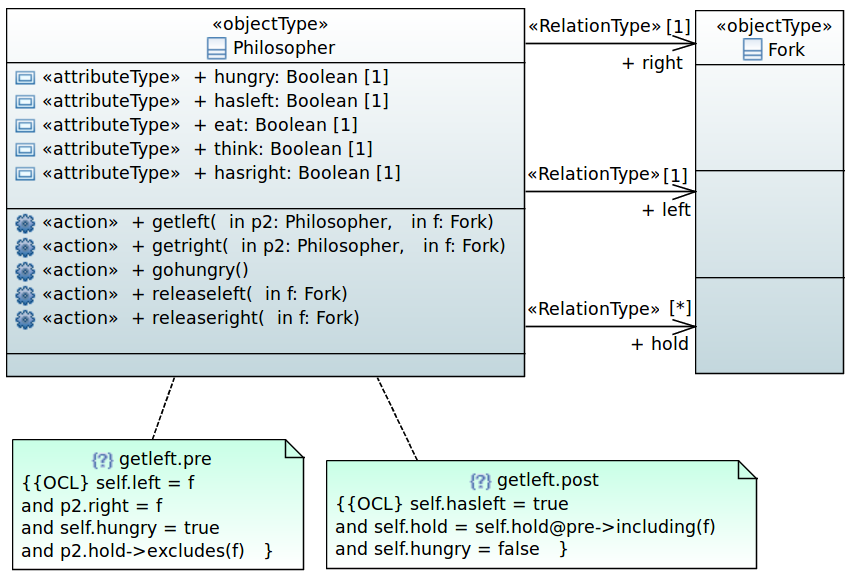
\includegraphics[width=0.8\linewidth]{a-philosophers-domain}
}

\newpage

\def\sname{3. Предметная область ``Мир кубиков''}
\section*{\sname}

\begin{mdframed}[style=excode] 
\begin{alltt}
\small
(define (domain blocks)
  (:requirements :strips :typing)
  (:types block)
  (:predicates (on ?x - block ?y - block)
           (ontable ?x - block)
           (clear ?x - block)
           (handempty)
           (holding ?x - block)
           )

  (:action pick-up
         :parameters (?x - block)
         :precondition (and (clear ?x) (ontable ?x) (handempty))
         :effect
         (and (not (ontable ?x))
           (not (clear ?x))
           (not (handempty))
           (holding ?x)))

  (:action put-down
         :parameters (?x - block)
         :precondition (holding ?x)
         :effect
         (and (not (holding ?x))
           (clear ?x)
           (handempty)
           (ontable ?x)))
  (:action stack
         :parameters (?x - block ?y - block)
         :precondition (and (holding ?x) (clear ?y))
         :effect
         (and (not (holding ?x))
           (not (clear ?y))
           (clear ?x)
           (handempty)
           (on ?x ?y)))
  (:action unstack
         :parameters (?x - block ?y - block)
         :precondition (and (on ?x ?y) (clear ?x) (handempty))
         :effect
         (and (holding ?x)
           (clear ?y)
           (not (clear ?x))
           (not (handempty))
           (not (on ?x ?y)))))
\end{alltt}
\end{mdframed}

\newpage
Задача для этой предметной области:\\

\begin{mdframed}[style=excode] 
\begin{alltt}
\small
(define (problem blocks-4-0)

(:domain blocks)

(:objects D B A C - block)

(:init  (clear C) 
    (clear A) 
    (clear B) 
    (clear D) 
    (ontable C) 
    (ontable A)
    (ontable B) 
    (ontable D) 
    (handempty))

(:goal (and (on D C) (on C B) (on B A)))
)
\end{alltt}
\end{mdframed}

Диаграмма фрагмента получившейся модели предметной области (по описанию задачи предположительная кратность [0],  интерактивно изменили на [0..1]):\\

\centerline{
    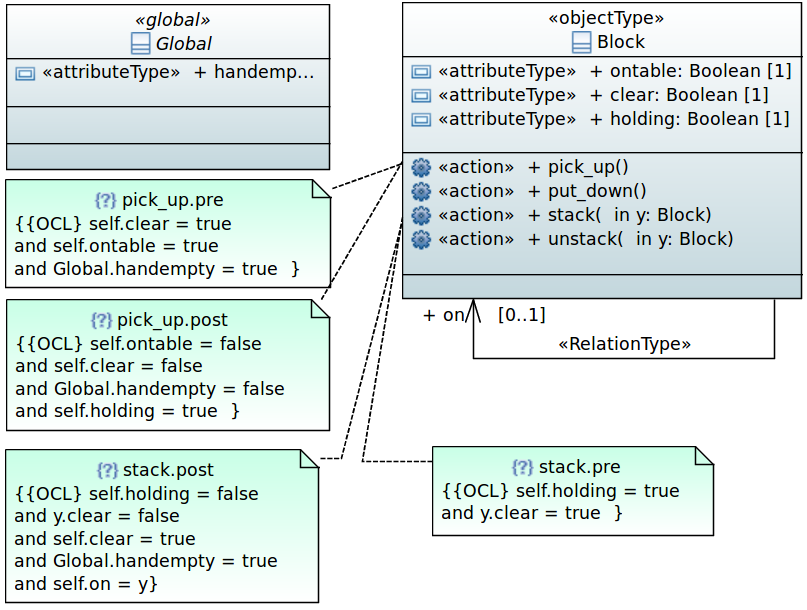
\includegraphics[width=0.8\linewidth]{a-blocks-domain}
}

\newpage
Диаграмма получившейся модели задачи планирования:\\

\centerline{
    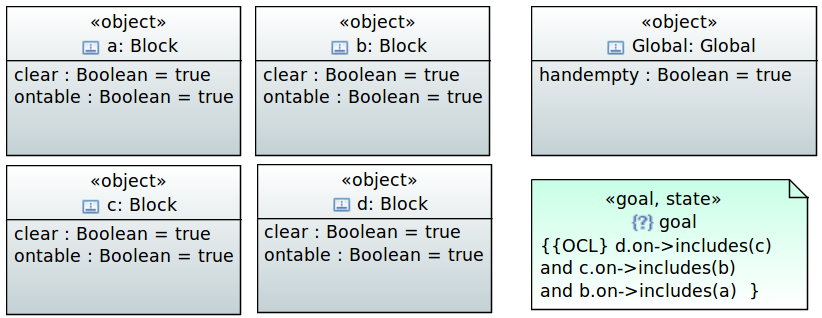
\includegraphics[width=0.8\linewidth]{a-blocks-problem}
}
